\chapter{Orthogonal Iteration}
\label{ch:orth-iter}

Supplementary reading:
\begin{itemize}
  \item \cite{TB} Lectures 24 and 28.
  \item \cite{Demmel} Section 4.4.3.
\end{itemize}

\section{Recap}

Last lecture (\Cref{ch:schur}) went from computing one eigenpair to asking what ``all eigenpairs'' should mean as a single object.
\begin{itemize}
  \item \emph{Deflation} (\Cref{sec:deflation}). Once $(\lambda_1, \vec{x}_1)$ is known, power iteration on $A - \lambda_1\vec{x}_1\vec{x}_1^\ast/(\vec{x}_1^\ast\vec{x}_1)$ finds the next eigenpair (Hermitian $A$, \Cref{prop:hotelling}).
  \item \emph{The need for subspace iteration} (\Cref{sec:subspace-motivation}). Deflation computes eigenpairs one after another, each with many Level 2 matrix-vector products. Iterating on a block of vectors at once turns them into Level 3 matrix-matrix products.
  \item \emph{Eigenvalues as matrix factorizations} (\Cref{sec:eig-factorization}). All eigenpairs together form the eigenvalue decomposition $A = X\Lambda X^{-1}$, but it need not exist: $N = \left[\begin{smallmatrix} 0 & 1 \\ 0 & 0 \end{smallmatrix}\right]$ sends $\vec{e}_2 \mapsto \vec{e}_1 \mapsto \zerovec$ and has only one eigenvector.
  \item \emph{Defective matrices and Jordan blocks} (\Cref{sec:defective,sec:jordan}). Every matrix has a Jordan form $A = SJS^{-1}$ with $J = \diag(J_1, \dots, J_k)$ and $J_\ell \in \C^{n_\ell \times n_\ell}$ having $\lambda_\ell$ on the diagonal and ones on the superdiagonal. It is discontinuous in $A$, and $S$ can be arbitrarily ill-conditioned (\Cref{ex:jordan-unstable}).
  \item \emph{Schur factorization} (\Cref{sec:schur-fact}). Every matrix can be written $A = QTQ^\ast$ with $Q$ unitary and $T$ upper triangular (\Cref{thm:schur}). This is the stable replacement for the Jordan form, and it is what eigenvalue algorithms compute.
\end{itemize}

\section{From Schur Factorization to Diagonalization}
\label{sec:normal}

The Schur factorization $A = QTQ^\ast$ always exists, but $T$ is only upper triangular. When is it actually a diagonalization, i.e., when is $T$ diagonal, so that $A = Q\Lambda Q^\ast$ with $Q$ unitary?

\begin{definition}[Normal Matrix]
  \label{def:normal}
  $A \in \K^{m \times m}$ is \emph{normal} if $AA^\ast = A^\ast A$.
\end{definition}

Hermitian ($A^\ast = A$), skew-Hermitian ($A^\ast = -A$), and unitary ($A^\ast = A^{-1}$) matrices are normal, since in each case $A^\ast$ is a function of $A$ and therefore commutes with it. The nilpotent $N = \left[\begin{smallmatrix} 0 & 1 \\ 0 & 0 \end{smallmatrix}\right]$ is not:
\begin{equation}
  NN^\ast = \begin{bmatrix} 1 & 0 \\ 0 & 0 \end{bmatrix} \ne \begin{bmatrix} 0 & 0 \\ 0 & 1 \end{bmatrix} = N^\ast N.
\end{equation}

\begin{theorem}[Normal Matrices Are Unitarily Diagonalizable]
  \label{thm:normal-diag}
  $A \in \K^{m \times m}$ is normal if and only if it has an orthogonal eigenvalue decomposition $A = Q\Lambda Q^\ast$ with $Q$ unitary and $\Lambda$ diagonal. In this case the triangular factor $T$ of every Schur factorization $A = QTQ^\ast$ is diagonal.
\end{theorem}

Over $\C$, an ``orthogonal'' eigenvalue decomposition means that the eigenvector matrix $Q$ is unitary.

\begin{proof}
  ($\Leftarrow$) If $A = Q\Lambda Q^\ast$, then $A^\ast = Q\overline{\Lambda}Q^\ast$, and since diagonal matrices commute,
  \begin{equation}
    AA^\ast = Q\Lambda\overline{\Lambda}Q^\ast = Q\overline{\Lambda}\Lambda Q^\ast = A^\ast A.
  \end{equation}

  ($\Rightarrow$) Take a Schur factorization $A = QTQ^\ast$ (\Cref{thm:schur}). Then
  \begin{equation}
    QTT^\ast Q^\ast = AA^\ast = A^\ast A = QT^\ast TQ^\ast,
  \end{equation}
  and multiplying by $Q^\ast$ on the left and $Q$ on the right gives $TT^\ast = T^\ast T$: the triangular factor is normal too. Now compare the $(1,1)$ entries. Since $T$ is upper triangular, its first column is $t_{11}\vec{e}_1$, while its first row is full:
  \begin{equation}
    (T^\ast T)_{11} = \sum_{i=1}^m\abs{t_{i1}}^2 = \abs{t_{11}}^2, \qquad (TT^\ast)_{11} = \sum_{i=1}^m\abs{t_{1i}}^2.
  \end{equation}
  Equating them gives $\sum_{i=2}^m\abs{t_{1i}}^2 = 0$, so $t_{1i} = 0$ for $i \ge 2$, and $T = \diag(t_{11}, T_2)$ with $T_2$ upper triangular. The lower right blocks of $TT^\ast = T^\ast T$ give $T_2T_2^\ast = T_2^\ast T_2$, so $T_2$ is again normal, and induction on $m$ shows that $T$ is diagonal. Hence $A = QTQ^\ast$ is an orthogonal eigenvalue decomposition.
\end{proof}

Pictorially, in terms of the shapes of the factors, the key identity says that lower times upper equals upper times lower.
\begin{center}
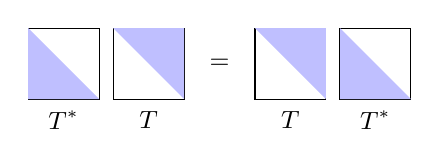
\begin{tikzpicture}[scale=0.9, every node/.style={font=\small}]
  \draw (0,0) rectangle (1,1); \fill[blue!25] (0,1) -- (0,0) -- (1,0) -- cycle;
  \node at (0.5,-0.3) {$T^\ast$};
  \draw (1.2,0) rectangle (2.2,1); \fill[blue!25] (1.2,1) -- (2.2,1) -- (2.2,0) -- cycle;
  \node at (1.7,-0.3) {$T$};
  \node at (2.7,0.5) {$=$};
  \draw (3.2,0) rectangle (4.2,1); \fill[blue!25] (3.2,1) -- (4.2,1) -- (4.2,0) -- cycle;
  \node at (3.7,-0.3) {$T$};
  \draw (4.4,0) rectangle (5.4,1); \fill[blue!25] (4.4,1) -- (4.4,0) -- (5.4,0) -- cycle;
  \node at (4.9,-0.3) {$T^\ast$};
\end{tikzpicture}
\end{center}
The $(1,1)$ entry of the left side sees only the first column of $T$, which is just $t_{11}$; the $(1,1)$ entry of the right side sees the whole first row. For the two to agree, the rest of the first row must vanish.

\section{Orthogonal Iteration}
\label{sec:orth-iter}

We now return to the question from \Cref{sec:subspace-motivation}: how do we run power iteration on several vectors at once without all of them collapsing onto $\vec{x}_1$? Throughout this section we assume that
\begin{equation}
  A \in \R^{m \times m} \text{ is diagonalizable}, \qquad \abs{\lambda_1} > \abs{\lambda_2} > \dots > \abs{\lambda_m}.
\end{equation}
Since non-real eigenvalues of a real matrix come in conjugate pairs of equal modulus, the strict ordering forces all eigenvalues, and hence all eigenvectors, to be real.

Suppose we want to compute $r = 2$ eigenpairs at once. We start by applying power iteration to two vectors simultaneously.
\begin{itemize}
  \item \emph{Problem.} Run independently, both vectors converge to the same vector $\vec{x}_1$ (up to sign), since almost every starting vector has a component along $\vec{x}_1$.
  \item \emph{Idea.} After each multiplication, project $\vec{q}_2$ onto the orthogonal complement of $\vec{q}_1$. Then $\vec{q}_2$ stays orthogonal to $\vec{q}_1$ and cannot converge to $\vec{x}_1$ as well.
\end{itemize}

\begin{algorithm}[H]
  \caption{Orthogonal iteration with two vectors.}
  \label{alg:orth-iter-2}
  \begin{algorithmic}[1]
    \State $\vec{q}_1, \vec{q}_2 \gets$ random vectors
    \While{not converged}
      \State $\vec{q}_1 \gets A\vec{q}_1$, \quad $\vec{q}_2 \gets A\vec{q}_2$
      \State $\vec{q}_2 \gets \left(I - \dfrac{\vec{q}_1\vec{q}_1^\ast}{\vec{q}_1^\ast\vec{q}_1}\right)\vec{q}_2$ \Comment{project out $\vec{q}_1$}
      \State $\vec{q}_1 \gets \vec{q}_1/\norm{\vec{q}_1}$, \quad $\vec{q}_2 \gets \vec{q}_2/\norm{\vec{q}_2}$
    \EndWhile
  \end{algorithmic}
\end{algorithm}

The last two lines are one step of Gram--Schmidt on $[A\vec{q}_1\ A\vec{q}_2]$, i.e., a reduced QR factorization of a two-column matrix (\Cref{ch:ls}). The first column is plain power iteration, so $\vec{q}_1 \to \pm\vec{x}_1/\norm{\vec{x}_1}$. Compare this with deflation (\Cref{sec:deflation}): there we projected out the \emph{converged} $\vec{x}_1$ at every step, here we project out the current approximation $\vec{q}_1$, so both vectors are iterated simultaneously.

\subsection{What Do the Two Vectors Converge To?}

Write $\vec{q}_i^{(k)}$ for the iterates after $k$ steps. The first vector is never touched by the projection, so
\begin{equation}
  \vec{q}_1^{(k)} = \frac{A^k\vec{q}_1^{(0)}}{\norm{A^k\vec{q}_1^{(0)}}}.
\end{equation}
That is, $\vec{q}_1$ performs plain power iteration (\Cref{alg:power}) and converges to $\vec{x}_1$, normalized and up to sign, at the rate $\abs{\lambda_2/\lambda_1}$.

For $\vec{q}_2$, assume that $\vec{q}_1 \approx \vec{x}_1$ already, with $\norm{\vec{x}_1} = 1$. Then the projection in \Cref{alg:orth-iter-2} is (approximately) a fixed matrix, and up to normalization
\begin{equation}
  \vec{q}_2^{(k)} \approx (I - \vec{x}_1\vec{x}_1^\ast)A\vec{q}_2^{(k-1)} = (I - \vec{x}_1\vec{x}_1^\ast)A(I - \vec{x}_1\vec{x}_1^\ast)\vec{q}_2^{(k-1)}.
\end{equation}
The equality holds because $\vec{q}_2^{(k-1)}$ was itself projected onto the orthogonal complement of $\vec{x}_1$ in the previous step, so inserting the projector once more changes nothing. So once $\vec{q}_1$ has converged, $\vec{q}_2$ performs power iteration with the matrix $(I - \vec{x}_1\vec{x}_1^\ast)A(I - \vec{x}_1\vec{x}_1^\ast)$.

\paragraph{The normal case.} For normal $A$ this matrix is exactly the Hotelling deflation of \Cref{prop:hotelling}:
\begin{equation}
  (I - \vec{x}_1\vec{x}_1^\ast)A(I - \vec{x}_1\vec{x}_1^\ast) = A - 2\lambda_1\vec{x}_1\vec{x}_1^\ast + \lambda_1\vec{x}_1\vec{x}_1^\ast = A - \lambda_1\vec{x}_1\vec{x}_1^\ast.
  \label{eq:orth-iter-deflation}
\end{equation}
To see the first equality, expand the product into four terms:
\begin{equation}
  A - \vec{x}_1(\vec{x}_1^\ast A) - (A\vec{x}_1)\vec{x}_1^\ast + \vec{x}_1(\vec{x}_1^\ast A\vec{x}_1)\vec{x}_1^\ast.
\end{equation}
We have $A\vec{x}_1 = \lambda_1\vec{x}_1$ and $\vec{x}_1^\ast A\vec{x}_1 = \lambda_1$. The remaining term needs normality: $\vec{x}_1$ is then also a \emph{left} eigenvector, $\vec{x}_1^\ast A = \lambda_1\vec{x}_1^\ast$. Indeed, $B \defeq A - \lambda_1I$ is normal along with $A$, and for any normal $B$ and any $\vec{v}$,
\begin{equation}
  \norm{B\vec{v}}^2 = \vec{v}^\ast B^\ast B\vec{v} = \vec{v}^\ast BB^\ast\vec{v} = \norm{B^\ast\vec{v}}^2,
\end{equation}
so $B\vec{x}_1 = \zerovec$ implies $B^\ast\vec{x}_1 = \zerovec$, i.e., $A^\ast\vec{x}_1 = \overline{\lambda_1}\vec{x}_1$; taking the conjugate transpose gives $\vec{x}_1^\ast A = \lambda_1\vec{x}_1^\ast$. Thus three of the four terms equal $\pm\lambda_1\vec{x}_1\vec{x}_1^\ast$.

So for normal $A$, $\vec{q}_2$ performs power iteration on the deflated matrix $A - \lambda_1\vec{x}_1\vec{x}_1^\ast$, whose eigenvalues are $0, \lambda_2, \dots, \lambda_m$. It converges to $\vec{x}_2$ at the rate $\abs{\lambda_3/\lambda_2}$. Orthogonal iteration does deflation automatically, without waiting for $\vec{x}_1$ to converge first.

\paragraph{The general case.} Without normality, $\vec{x}_1^\ast A \ne \lambda_1\vec{x}_1^\ast$ in general, and the deflated matrix is no longer $A - \lambda_1\vec{x}_1\vec{x}_1^\ast$. We can still find its eigenpairs by applying it to the eigenvectors of $A$. Write $P \defeq I - \vec{x}_1\vec{x}_1^\ast$. For every $i$,
\begin{equation}
  PAP\vec{x}_i = P\bigl(\lambda_i\vec{x}_i - \lambda_1\vec{x}_1(\vec{x}_1^\ast\vec{x}_i)\bigr) = \lambda_iP\vec{x}_i,
\end{equation}
since $P\vec{x}_1 = \zerovec$. Grouping the left side as $[PA](P\vec{x}_i)$, the operator $PA$ applied to the vector $P\vec{x}_i$, the identity says $PA(P\vec{x}_i) = \lambda_i(P\vec{x}_i)$ directly. (Read as $PAP$ applied to $\vec{x}_i$, one uses $P^2 = P$ to get $PAP(P\vec{x}_i) = \lambda_i(P\vec{x}_i)$ as well.) Hence the eigenpairs of $PA = (I - \vec{x}_1\vec{x}_1^\ast)A$ (and of $PAP$) are
\begin{equation}
  (0, \vec{x}_1) \qquad\text{and}\qquad (\lambda_i, P\vec{x}_i), \quad i = 2, \dots, m.
\end{equation}
Here $P\vec{x}_i = \vec{x}_i - (\vec{x}_1^\ast\vec{x}_i)\vec{x}_1 \ne \zerovec$ for $i \ge 2$, because the $\vec{x}_i$ are linearly independent. In words: the projection keeps the eigenvalues $\lambda_2, \dots, \lambda_m$, but replaces each eigenvector $\vec{x}_i$ by its component orthogonal to $\vec{x}_1$. In the normal case $\vec{x}_i \perp \vec{x}_1$, so $P\vec{x}_i = \vec{x}_i$, consistent with \cref{eq:orth-iter-deflation}.

\paragraph{Conclusion.} Once $\vec{q}_1$ has converged, $\vec{q}_2$ performs power iteration with $PA$, whose dominant eigenpair is $(\lambda_2, P\vec{x}_2)$ and whose next largest eigenvalue in modulus is $\lambda_3$. Hence, normalized and up to sign,
\begin{equation}
  \vec{q}_2^{(k)} \longrightarrow (I - \vec{x}_1\vec{x}_1^\ast)\vec{x}_2,
\end{equation}
at the rate $\abs{\lambda_3/\lambda_2}$. This is \emph{not} $\vec{x}_2$ unless $\vec{x}_1 \perp \vec{x}_2$, as for normal $A$. The two vectors cannot both be eigenvectors in general, since $\vec{q}_1 \perp \vec{q}_2$ by construction while $\vec{x}_1, \vec{x}_2$ need not be orthogonal.

What does converge is the subspace: $P\vec{x}_2 = \vec{x}_2 - (\vec{x}_1^\ast\vec{x}_2)\vec{x}_1$, so
\begin{equation}
  \spn(\vec{q}_1, \vec{q}_2) \longrightarrow \spn(\vec{x}_1, \vec{x}_2),
\end{equation}
an invariant subspace of $A$, and $\vec{q}_1, \vec{q}_2$ is an orthonormal basis of it whose first vector is an eigenvector. These are exactly the first two columns of a Schur factorization (\Cref{sec:schur-fact}): $A\vec{q}_1 = \lambda_1\vec{q}_1$ and $A\vec{q}_2 \in \spn(\vec{q}_1, \vec{q}_2)$, so $T$ is upper triangular in its first two columns.

\subsection{Extracting the Eigenvalues}

Orthogonal iteration gives an orthonormal basis of $\spn(\vec{x}_1, \vec{x}_2)$, but $\vec{q}_2$ is not an eigenvector. How do we find the eigenvalues? Collect the iterates into a tall matrix with orthonormal columns and compress $A$ onto their span:
\begin{equation}
  Q_k \defeq \begin{bmatrix} \vec{q}_1^{(k)} & \vec{q}_2^{(k)} \end{bmatrix} \in \K^{m \times 2}, \qquad Q_k^\ast AQ_k \in \K^{2 \times 2}.
\end{equation}

\begin{proposition}[Projected Matrix]
  \label{prop:orth-iter-2x2}
  As $k \to \infty$,
  \begin{equation}
    Q_k^\ast AQ_k = \begin{bmatrix} \vec{q}_1^\ast A\vec{q}_1 & \vec{q}_1^\ast A\vec{q}_2 \\ \vec{q}_2^\ast A\vec{q}_1 & \vec{q}_2^\ast A\vec{q}_2 \end{bmatrix} \longrightarrow \begin{bmatrix} \lambda_1 & \ast \\ 0 & \lambda_2 \end{bmatrix}.
  \end{equation}
\end{proposition}

In terms of shapes: a $2 \times m$ matrix times an $m \times m$ matrix times an $m \times 2$ matrix gives a $2 \times 2$ upper triangular matrix with the two dominant eigenvalues on its diagonal.
\begin{center}
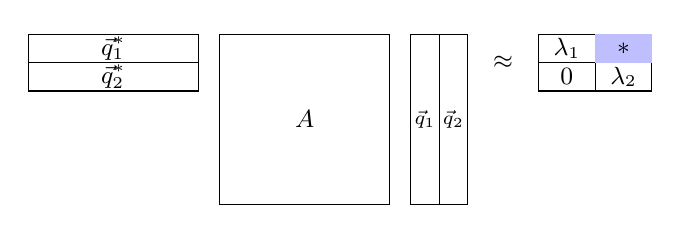
\begin{tikzpicture}[scale=0.9, every node/.style={font=\small}]
  \draw (0,1.6) rectangle (2.4,2.4); \draw (0,2.0) -- (2.4,2.0);
  \node at (1.2,2.2) {$\vec{q}_1^\ast$}; \node at (1.2,1.8) {$\vec{q}_2^\ast$};
  \draw (2.7,0) rectangle (5.1,2.4); \node at (3.9,1.2) {$A$};
  \draw (5.4,0) rectangle (6.2,2.4); \draw (5.8,0) -- (5.8,2.4);
  \node[font=\scriptsize] at (5.6,1.2) {$\vec{q}_1$}; \node[font=\scriptsize] at (6.0,1.2) {$\vec{q}_2$};
  \node at (6.7,2.0) {$\approx$};
  \draw (7.2,1.6) rectangle (8.8,2.4); \draw (8.0,1.6) -- (8.0,2.4); \draw (7.2,2.0) -- (8.8,2.0);
  \fill[blue!25] (8.0,2.0) rectangle (8.8,2.4);
  \node at (7.6,2.2) {$\lambda_1$}; \node at (8.4,2.2) {$\ast$};
  \node at (7.6,1.8) {$0$}; \node at (8.4,1.8) {$\lambda_2$};
\end{tikzpicture}
\end{center}

\begin{proof}[Proof sketch]
  Write $Q = Q_k$ and assume $k$ is large, so that $\vec{q}_1 \approx \vec{x}_1$ and $\spn(\vec{q}_1, \vec{q}_2) \approx \spn(\vec{x}_1, \vec{x}_2)$.

  \emph{The $(2,1)$ entry vanishes.} Using $\vec{q}_1 \approx \vec{x}_1$ twice,
  \begin{equation}
    \vec{q}_2^\ast A\vec{q}_1 \approx \vec{q}_2^\ast A\vec{x}_1 = \lambda_1\vec{q}_2^\ast\vec{x}_1 \approx \lambda_1\vec{q}_2^\ast\vec{q}_1 = 0.
  \end{equation}

  \emph{The eigenvalues are $\lambda_1, \lambda_2$.} For $i = 1, 2$, the eigenvector $\vec{x}_i$ lies (approximately) in $\range(Q)$, so there is $\vec{v}_i \in \K^2$ with $Q\vec{v}_i = \vec{x}_i$. Then, using $Q^\ast Q = I_2$,
  \begin{equation}
    Q^\ast AQ\vec{v}_i = Q^\ast A\vec{x}_i = \lambda_iQ^\ast\vec{x}_i \approx \lambda_iQ^\ast Q\vec{v}_i = \lambda_i\vec{v}_i.
  \end{equation}
  So $(\lambda_i, \vec{v}_i)$ are the eigenpairs of the $2 \times 2$ matrix $Q^\ast AQ$.

  \emph{Order on the diagonal.} The $(1,1)$ entry $\vec{q}_1^\ast A\vec{q}_1$ is the Rayleigh quotient of $\vec{q}_1 \approx \vec{x}_1$, so it tends to $\lambda_1$. A triangular matrix has its eigenvalues on the diagonal, so the $(2,2)$ entry tends to $\lambda_2$.
\end{proof}

The proof also shows how to get eigenvectors back. Solve the small eigenvalue problem $Q_k^\ast AQ_k\vec{v}_i = \lambda_i\vec{v}_i$ and lift: $\vec{x}_i \approx Q_k\vec{v}_i$. The $(1,2)$ entry $\ast$ is in general nonzero: by the computation $A\vec{q}_2 = \lambda_2\vec{q}_2 + \beta\vec{q}_1$, it equals $\beta = (\lambda_2 - \lambda_1)(\vec{x}_1^\ast\vec{x}_2)/\norm{P\vec{x}_2}$ in the limit, which vanishes exactly when $\vec{x}_1 \perp \vec{x}_2$.

\section{Orthogonal Iteration in General}
\label{sec:orth-iter-general}

To compute $r > 2$ eigenpairs at once, start with $r$ random vectors, the columns of $Q \in \K^{m \times r}$. Multiplying by $A$ is one matrix-matrix product, and the Gram--Schmidt step of \Cref{alg:orth-iter-2} becomes a reduced QR factorization, which orthonormalizes all $r$ columns at once.

\begin{algorithm}[H]
  \caption{Orthogonal iteration.}
  \label{alg:orth-iter}
  \begin{algorithmic}[1]
    \Require $A \in \K^{m \times m}$, starting $Q \in \K^{m \times r}$ (e.g., random)
    \For{$k = 1, \dots, \mathrm{iters}$}
      \State $Z \gets AQ$ \Comment{Level 3: $A$ is read once for all $r$ columns}
      \State $QR \gets Z$ \Comment{reduced QR, $Q \in \K^{m \times r}$}
    \EndFor
  \end{algorithmic}
\end{algorithm}

Column $j$ of the QR factorization is $A\vec{q}_j$ with its components along $\vec{q}_1, \dots, \vec{q}_{j-1}$ removed, so the first two columns do exactly what \Cref{alg:orth-iter-2} does, and column $j$ is power iteration projected onto the orthogonal complement of the first $j - 1$ columns.

\begin{remark}[Julia]
  The naive loop body \texttt{Q = A*Q; Q, R = qr(Q)} goes wrong in Julia: \texttt{qr} returns $Q$ in the implicit form of \Cref{ch:qr}, which acts as the full $m \times m$ matrix, so from the second iteration on \texttt{A*Q} is $m \times m$. Ask for the thin factor explicitly:
\begin{lstlisting}
for k = 1:iters
    Q = Matrix(qr(A*Q).Q)   # m x r
end
\end{lstlisting}
\end{remark}

\section{Convergence of Eigenvector Estimates}
\label{sec:orth-iter-eigvec}

Run \Cref{alg:orth-iter} with $r$ columns and write $Q_k = [\vec{q}_1^{(k)} \cdots \vec{q}_r^{(k)}]$ for the iterate after $k$ steps. The first $i$ columns of a QR factorization depend only on the first $i$ columns of the factored matrix, so the first $i$ columns of $Q_k$ are exactly what orthogonal iteration with $i$ vectors would produce. Running \Cref{alg:orth-iter} with $r$ columns therefore runs it with $1, 2, \dots, r$ columns at the same time, and the argument of \Cref{sec:orth-iter} generalizes to
\begin{equation}
  \spn\bigl(\vec{q}_1^{(k)}, \dots, \vec{q}_i^{(k)}\bigr) \longrightarrow \spn(\vec{x}_1, \dots, \vec{x}_i), \qquad i = 1, \dots, r.
  \label{eq:orth-iter-nested}
\end{equation}
A proof via $\spn(Q_k) = \spn(A^kQ_0)$ is given in \Cref{sec:orth-iter-conv}.

\paragraph{Eigenvalues.} By the same argument as in the proof of \Cref{prop:orth-iter-2x2}, for $i \le r$ the eigenvector $\vec{x}_i$ lies (approximately) in $\range(Q_k)$, so $Q_k\vec{v}_i \approx \vec{x}_i$ for some $\vec{v}_i \in \K^r$, and
\begin{equation}
  Q_k^\ast AQ_k\vec{v}_i \approx Q_k^\ast A\vec{x}_i = \lambda_iQ_k^\ast\vec{x}_i \approx \lambda_iQ_k^\ast Q_k\vec{v}_i = \lambda_i\vec{v}_i.
\end{equation}
So the eigenvalues of the $r \times r$ matrix $Q_k^\ast AQ_k$ converge to $\lambda_1, \dots, \lambda_r$, and $Q_k\vec{v}_i$ approximates $\vec{x}_i$. What about the columns of $Q_k$ themselves?

\paragraph{The symmetric (normal) case.} If $A$ is symmetric, or more generally normal, then as before $\vec{q}_1^{(k)} \to \vec{x}_1$ and $\vec{q}_2^{(k)} \to \vec{x}_2$, up to sign. The same argument applies to every column. Once $\vec{q}_1, \dots, \vec{q}_{i-1}$ have converged to the orthonormal eigenvectors $\vec{x}_1, \dots, \vec{x}_{i-1}$, column $i$ performs power iteration with
\begin{equation}
  P_{i-1}A, \qquad P_{i-1} \defeq I - \sum_{j < i}\vec{x}_j\vec{x}_j^\ast,
\end{equation}
and for normal $A = \sum_j\lambda_j\vec{x}_j\vec{x}_j^\ast$ this is $\sum_{j \ge i}\lambda_j\vec{x}_j\vec{x}_j^\ast$, with dominant eigenpair $(\lambda_i, \vec{x}_i)$. Hence
\begin{equation}
  \vec{q}_i^{(k)} \longrightarrow \pm\vec{x}_i, \qquad 1 \le i \le r,
\end{equation}
at the rate $\abs{\lambda_{i+1}/\lambda_i}$. For normal $A$, orthogonal iteration delivers the eigenvectors directly.

\paragraph{The non-normal case.} Now let $A = X\Lambda X^{-1}$ be diagonalizable, but not normal. The eigenvectors are no longer orthogonal, while the columns of $Q_k$ are, so they cannot converge to the $\vec{x}_i$. To identify their limit, take a reduced QR factorization of the first $r$ eigenvectors,
\begin{equation}
  [\vec{x}_1 \cdots \vec{x}_r] \eqqcolon Q^XR^X, \qquad Q^X = [\vec{q}_1^X \cdots \vec{q}_r^X] \in \K^{m \times r}, \quad R^X \in \K^{r \times r} \text{ upper triangular}.
  \label{eq:orth-iter-QX}
\end{equation}
Since the $\vec{x}_i$ are linearly independent, $R^X$ is invertible, and as in \cref{eq:schur-nested},
\begin{equation}
  \spn(\vec{q}_1^X, \dots, \vec{q}_i^X) = \spn(\vec{x}_1, \dots, \vec{x}_i), \qquad i = 1, \dots, r.
\end{equation}
In other words, $Q^X$ is the result of Gram--Schmidt applied to $\vec{x}_1, \dots, \vec{x}_r$. For example, $\vec{q}_2^X$ is $(I - \vec{q}_1^X\vec{q}_1^{X\ast})\vec{x}_2$ normalized, which is exactly the limit of $\vec{q}_2^{(k)}$ found in \Cref{sec:orth-iter}.

\begin{proposition}[Limit of the Orthogonal Iterates]
  \label{prop:orth-iter-QX}
  Let $A \in \R^{m \times m}$ be diagonalizable with $\abs{\lambda_1} > \dots > \abs{\lambda_m}$, and assume that \cref{eq:orth-iter-nested} holds. Then $Q_k \to Q^X$ up to the signs of the columns: $\vec{q}_i^{(k)} \mp \vec{q}_i^X \to \zerovec$ for $i = 1, \dots, r$, with the sign chosen at each step $k$.
\end{proposition}

\begin{proof}[Proof sketch]
  We check column by column, writing $\vec{q}_i$ for the limit of $\vec{q}_i^{(k)}$ (up to sign). For the first column, $\vec{q}_1^{(k)}$ performs power iteration, so $\vec{q}_1 = \pm\vec{x}_1/\norm{\vec{x}_1} = \pm\vec{q}_1^X$.

  For the second column, \cref{eq:orth-iter-nested} gives
  \begin{equation}
    \spn(\vec{x}_1, \vec{x}_2) = \spn(\vec{q}_1, \vec{q}_2) = \spn(\vec{q}_1^X, \vec{q}_2^X) \eqqcolon S_2.
  \end{equation}
  Now $\vec{q}_2$ is a unit vector in the orthogonal complement of $\vec{q}_1$ in $S_2$, and $\vec{q}_2^X$ is a unit vector in the orthogonal complement of $\vec{q}_1^X = \pm\vec{q}_1$ in $S_2$. This complement is one-dimensional, since $S_2$ is two-dimensional. A real one-dimensional space contains exactly two unit vectors, so $\vec{q}_2 = \pm\vec{q}_2^X$.

  Repeating the argument with
  \begin{equation}
    \spn(\vec{x}_1, \dots, \vec{x}_i) = \spn(\vec{q}_1, \dots, \vec{q}_i) = \spn(\vec{q}_1^X, \dots, \vec{q}_i^X) \eqqcolon S_i,
  \end{equation}
  both $\vec{q}_i$ and $\vec{q}_i^X$ are unit vectors in the orthogonal complement of $\spn(\vec{q}_1, \dots, \vec{q}_{i-1}) = \spn(\vec{q}_1^X, \dots, \vec{q}_{i-1}^X)$ in $S_i$, which is one-dimensional. Hence $\vec{q}_i = \pm\vec{q}_i^X$ for all $i \le r$.
\end{proof}

Over $\C$ the same argument determines each column up to a factor $e^{\mathrm{i}\theta}$ instead of a sign. For normal $A$ the normalized eigenvectors are orthonormal, so $Q^X$ consists of the normalized $\vec{x}_i$ themselves (up to sign), and \Cref{prop:orth-iter-QX} reduces to $\vec{q}_i^{(k)} \to \pm\vec{x}_i$, as above.

\section{Convergence to Schur Factorization}
\label{sec:orth-iter-schur}

Now take $r = m$, so that $Q_k$ and $Q^X$ are square and orthogonal, and consider the projected matrix
\begin{equation}
  T_k \defeq Q_k^\ast AQ_k \longrightarrow Q^{X\ast}AQ^X,
\end{equation}
where the limit holds up to signs, as discussed below. To evaluate the limit, use \cref{eq:orth-iter-QX}, now with $X = [\vec{x}_1 \cdots \vec{x}_m]$:
\begin{equation}
  Q^XR^X = X \quad\Longleftrightarrow\quad Q^X = X(R^X)^{-1} \quad\Longleftrightarrow\quad Q^{X\ast} = (Q^X)^{-1} = R^XX^{-1}.
\end{equation}
Hence
\begin{equation}
  Q^{X\ast}AQ^X = R^XX^{-1}AX(R^X)^{-1} = R^XX^{-1}X\Lambda(R^X)^{-1} = \underbrace{R^X\Lambda(R^X)^{-1}}_{\text{upper triangular}}.
  \label{eq:orth-iter-schur-limit}
\end{equation}
The product of upper triangular matrices is upper triangular, and its diagonal is $r_{ii}\lambda_ir_{ii}^{-1} = \lambda_i$. So $A = Q^X\bigl(R^X\Lambda(R^X)^{-1}\bigr)Q^{X\ast}$ is a Schur factorization of $A$ (\Cref{thm:schur}), with the eigenvalues on the diagonal in decreasing order of modulus. The eigenpairs of the triangular factor are
\begin{equation}
  \bigl(\lambda_i, R^X\vec{e}_i\bigr), \qquad\text{since}\quad R^X\Lambda(R^X)^{-1}R^X\vec{e}_i = R^X\Lambda\vec{e}_i = \lambda_iR^X\vec{e}_i,
\end{equation}
and lifting them back gives the eigenvectors of $A$, $Q^XR^X\vec{e}_i = X\vec{e}_i = \vec{x}_i$. (The eigenvector is $R^X\vec{e}_i$, the $i$th column of $R^X$, and not $(R^X)^{-1}\vec{e}_i$; only the former is mapped to $\vec{x}_i$ by $Q^X$.)

The signs do not affect this picture. If $Q_k \approx Q^XD$ with $D = \diag(\pm 1)$, then $T_k \approx D\,R^X\Lambda(R^X)^{-1}D$, which is still upper triangular with the same diagonal; only some entries above the diagonal change sign.

In summary: for every $k$, $A = Q_kT_kQ_k^\ast$ exactly, with $Q_k$ orthogonal, and the factor $T_k = Q_k^\ast AQ_k$ converges to an upper triangular matrix. So
\begin{equation}
  Q_k, \quad Q_k^\ast AQ_k, \quad Q_k^\ast
\end{equation}
converge to the Schur factorization of $A$, and we can read off the eigenvalues from the diagonal of $Q_k^\ast AQ_k$. The precise conditions on the starting matrix, and a proof that does not presuppose \cref{eq:orth-iter-nested}, are in \Cref{thm:orth-iter-schur}.

Computing $T_{k+1}$ this way requires $Q_k$ and a matrix-matrix product with $A$ in every step. \Cref{sec:basic-qr} derives an iteration $T_k \to T_{k+1}$ that works with $T_k$ alone, the QR algorithm, and \Cref{ch:hessenberg-qr} makes each of its steps cheap by first reducing $A$ to Hessenberg form.

\section{(SUPPLEMENT) Further Topics}
\label{sec:orth-iter-supp}

\paragraph{More consequences of normality.} Let $A = Q\Lambda Q^\ast$ be normal and write $\lambda_i = \abs{\lambda_i}e^{\mathrm{i}\theta_i}$. Then $A = \bigl(Q\diag(e^{\mathrm{i}\theta_i})\bigr)\abs{\Lambda}Q^\ast$ is an SVD up to the ordering of the entries, so the singular values of a normal matrix are the moduli of its eigenvalues~\cite[Lecture~24]{TB}. In particular $\norm{A}_2 = \max_i\abs{\lambda_i}$ and $\norm{A^k}_2 = \max_i\abs{\lambda_i}^k$: powers of a normal matrix show none of the transient growth of a Jordan block (\Cref{sec:jordan}). The Schur form also measures how far a general $A$ is from normal. Write the triangular factor as $T = \Lambda + N$ with $N$ strictly upper triangular. Since the Frobenius norm is unitarily invariant,
\begin{equation}
  \norm{A}_F^2 = \norm{T}_F^2 = \sum_{i=1}^m\abs{\lambda_i}^2 + \norm{N}_F^2.
\end{equation}
Hence $\sum_i\abs{\lambda_i}^2 \le \norm{A}_F^2$, with equality if and only if $N = 0$, i.e., if and only if $A$ is normal (\Cref{thm:normal-diag}). The quantity $\norm{N}_F$, the \emph{departure from normality}, does not depend on which Schur factorization is chosen, since $\norm{A}_F$ and the eigenvalues do not.

\paragraph{The Rayleigh--Ritz procedure.} The projected matrix $H \defeq Q^\ast AQ$ of \Cref{prop:orth-iter-2x2}, for any $Q \in \K^{m \times r}$ with orthonormal columns, generalizes the Rayleigh quotient from one vector to a subspace. Its eigenvalues $\theta_i$ are called \emph{Ritz values}, and the lifted eigenvectors $Q\vec{v}_i$ \emph{Ritz vectors}. The choice $R = H$ minimizes the residual $\norm{AQ - QR}_2$ over all $R \in \K^{r \times r}$: with $E \defeq AQ - QH$ we have $Q^\ast E = 0$, so for every $\vec{y}$,
\begin{equation}
  \norm{(AQ - QR)\vec{y}}^2 = \norm{E\vec{y} + Q(H - R)\vec{y}}^2 = \norm{E\vec{y}}^2 + \norm{(H - R)\vec{y}}^2 \ge \norm{E\vec{y}}^2.
\end{equation}
For Hermitian $A$ there are $r$ eigenvalues of $A$, not necessarily the largest ones, each within $\norm{E}_2$ of a different Ritz value~\cite[\S7.2]{Demmel}. In subspace iteration for Hermitian matrices one therefore often replaces $Q_k$ by its Ritz vectors $Q_kV$, where $Q_k^\ast AQ_k = V\Theta V^\ast$. These depend only on $\spn(Q_k) = \spn(A^kQ_0)$, in which the components along $\vec{x}_j$, $j > r$, are damped relative to $\vec{x}_i$ by roughly $\abs{\lambda_j/\lambda_i}^k \le \abs{\lambda_{r+1}/\lambda_i}^k$. So the $i$th Ritz vector converges like $\abs{\lambda_{r+1}/\lambda_i}^k$ rather than $\abs{\lambda_{i+1}/\lambda_i}^k$, and iterating with a few more columns than eigenpairs wanted speeds up convergence. Without the Rayleigh--Ritz step, extra columns do not help the first ones, since the leading columns of \Cref{alg:orth-iter} never see the later ones.

\paragraph{Convergence of the individual entries.} The leading $p$ columns span a subspace converging at the rate $\abs{\lambda_{p+1}/\lambda_p}$, so the block $(T_k)_{p+1:m,\,1:p}$ decays like $\abs{\lambda_{p+1}/\lambda_p}^k$. The diagonal entry $(T_k)_{pp}$ is affected by the blocks on both sides of it, and converges to $\lambda_p$ like
\begin{equation}
  \max\left(\abs{\frac{\lambda_{p+1}}{\lambda_p}}, \abs{\frac{\lambda_p}{\lambda_{p-1}}}\right)^k,
\end{equation}
where only the first ratio is present for $p = 1$ and only the second for $p = m$~\cite[\S4.4.3]{Demmel}. A pair of eigenvalues of nearly equal modulus thus slows down only the part of $T_k$ near their position, while the rest of the Schur form converges quickly. For symmetric $A$, all columns of $Q_k$ converge to eigenvectors linearly with constant $\max_{1 \le j \le r}\abs{\lambda_{j+1}/\lambda_j}$~\cite[Thm.~28.1]{TB}.

\paragraph{Why orthonormalize at every step.} Mathematically, $\spn(Q_k) = \spn(A^kQ_0)$, so we could compute $V_k = A^kQ_0$ and orthonormalize once at the end (``unnormalized simultaneous iteration''). In floating point this fails: every column of $A^kQ_0$ converges to a multiple of $\vec{x}_1$, so the columns become nearly parallel, and the information about $\vec{x}_2, \dots, \vec{x}_r$ sits in components that are smaller by factors $\abs{\lambda_i/\lambda_1}^k$ and are lost to rounding errors~\cite[Lecture~28]{TB}. Orthonormalizing after every multiplication keeps a well-conditioned basis of the same subspace. With $Q_0 = I$ and $r = m$, the accumulated triangular factors give the QR factorization of $A^k$ itself; this identity is the starting point of the QR algorithm in \Cref{ch:qr-alg}.

\paragraph{Beyond subspace iteration.} Each step of orthogonal iteration costs one product $AQ$, about $2m^2r$ flops for dense $A$ and far less for sparse $A$, plus $O(mr^2)$ for the QR factorization, so it is attractive when only a few dominant eigenpairs of a large sparse matrix are needed. Its convergence is still linear with the ratio $\abs{\lambda_{r+1}/\lambda_r}$. Krylov methods do better with the same products: instead of keeping only $A^kQ_0$, they apply Rayleigh--Ritz to the whole Krylov subspace $\spn(\vec{q}, A\vec{q}, \dots, A^{k-1}\vec{q})$, which contains all earlier power iterates. This leads to the Arnoldi iteration and, for Hermitian $A$, the Lanczos iteration~\cite[Lectures~33, 34, and~36]{TB}, \cite[Chapter~7]{Demmel}.
